\section{The Elementary Six-Gap Phase Slip}
\label{sec:elementary-g6}

\subsection{The bilateral interface and its essential spectrum}
\label{subsec:bilateral-interface-essential-spectrum}

The elementary interface replaces one reference gap of length four by a gap
of length six.  On \(\mathbb Z\), let
\[
D_6=\{-4j:j\geq0\}\cup\{6+4j:j\geq0\}
\]
and set \(Q_i^{(6)}=+1\) for \(i\in D_6\). Choose the lift
\(\tau_0^{(6)}=1\) and
\(\tau_{i+1}^{(6)}=Q_i^{(6)}\tau_i^{(6)}\).  We write
\[
(A_6u)_i=u_{i-1}+u_{i+1}
+\tau_{i-2}^{(6)}u_{i-2}+\tau_i^{(6)}u_{i+2},
\qquad H_6=A_6^2.
\]
The other lift has the same squared spectrum by
equation~\eqref{eq:lift-negation}; reflection gives the opposite interface
orientation.  The left tail has positive \(Q\)-sites \(4\mathbb Z\), while
the right tail has positive sites \(6+4\mathbb Z\).  They are translates
\(B_0\) and \(B_2\) of the reference phase.

Figure~\ref{fig:reference-g6} shows the positive \(Q\)-sites of the reference
bulk and the bilateral \(B_0\)-to-\(B_2\) interface; black sites represent
\(Q_i=+1\).
\begin{figure}[t]
\centering
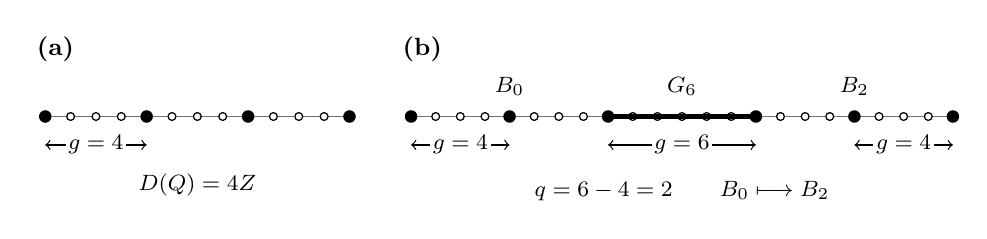
\begin{tikzpicture}[
  x=0.92cm,
  y=0.82cm,
  line cap=round,
  line join=round,
  positive/.style={circle,fill=black,inner sep=1.6pt},
  negative/.style={circle,draw=black,fill=white,inner sep=1.0pt,
    line width=0.45pt},
  bulk/.style={draw=black!55,line width=0.65pt},
  defect/.style={draw=black,line width=1.55pt},
  panel/.style={font=\small\bfseries,anchor=west},
  label/.style={font=\footnotesize,align=center}
]
  % (a) Period-eight reference bulk.
  \node[panel] at (0,2.62) {(a)};
  \draw[bulk] (0.25,1.58)--(4.45,1.58);
  \foreach \i in {0,...,12} {
    \pgfmathtruncatemacro{\r}{mod(\i,4)}
    \ifnum\r=0
      \node[positive] at ({0.25+0.35*\i},1.58) {};
    \else
      \node[negative] at ({0.25+0.35*\i},1.58) {};
    \fi
  }
  \draw[<->,line width=0.45pt]
    (0.25,1.14)--node[label,fill=white,inner sep=1pt]
    {$g=4$} (1.65,1.14);
  \node[label] at (2.35,0.52) {$D(Q)=4\mathbb Z$};

  % (b) Bilateral six-gap phase slip with gaps 4,4,6,4,4.
  \node[panel] at (5.05,2.62) {(b)};
  \draw[bulk] (5.30,1.58)--(12.78,1.58);
  \foreach \i in {0,...,22} {
    \node[negative] at ({5.30+0.34*\i},1.58) {};
  }
  \foreach \i in {0,4,8,14,18,22} {
    \node[positive] at ({5.30+0.34*\i},1.58) {};
  }
  \draw[defect] (8.02,1.58)--(10.06,1.58);
  \node[label] at (6.66,2.05) {$B_0$};
  \node[label] at (9.04,2.05) {$G_6$};
  \node[label] at (11.42,2.05) {$B_2$};
  \draw[<->,line width=0.45pt]
    (5.30,1.14)--node[label,fill=white,inner sep=1pt]
    {$g=4$} (6.66,1.14);
  \draw[<->,line width=0.45pt]
    (8.02,1.14)--node[label,fill=white,inner sep=1pt]
    {$g=6$} (10.06,1.14);
  \draw[<->,line width=0.45pt]
    (11.42,1.14)--node[label,fill=white,inner sep=1pt]
    {$g=4$} (12.78,1.14);
  \node[label] at (9.04,0.42)
    {$q=6-4=2$\qquad $B_0\longmapsto B_2$};
\end{tikzpicture}

\caption{The period-eight reference bulk and the elementary six-gap phase
slip.}
\label{fig:reference-g6}
\end{figure}

Every row of \(A_6\) has four entries of absolute value one, and the matrix is
real symmetric.  Hence \(A_6\) is bounded and self-adjoint,
\(\|A_6\|\leq4\), and
\[
0\leq H_6\leq16I.
\]

\begin{lemma}[Essential spectrum and tail matching]
\label{lem:g6-essential}
The G6 squared operator satisfies
\[
\operatorname{Spec}_{\mathrm{ess}}(H_6)
=\operatorname{Spec}(H_{\mathrm{ref}}),
\qquad
\sup\operatorname{Spec}_{\mathrm{ess}}(H_6)=\eta.
\]
Every \(y>\eta\) in \(\operatorname{Spec}(H_6)\) is an isolated eigenvalue
of finite multiplicity.  Its nonzero unsquared components decay
exponentially on both periodic tails and obey the stable/unstable matching
criterion at \(\lambda=\pm\sqrt y\).  The next subsection writes the positive
branch explicitly; the \(K\)-symmetry below identifies the negative branch.
\end{lemma}

\begin{proof}
Choose two cuts outside the finite interface core.  Decoupling at those cuts
gives the direct sum of a left periodic half-line compression, a finite
middle block, and a right periodic half-line compression.  Since \(H_6\)
has range four, its difference from this decoupled operator has finite rank.
The finite block contributes no essential spectrum.

For completeness, a periodic half-line compression has the same essential
spectrum as its whole-line operator.  In one direction, a whole-line Bloch
solution cut off on \(L\) cells far down the half-line has norm of order
\(L^{1/2}\), while the residual is confined to a fixed number of boundary
sites.  Normalization and Weyl's criterion put every whole-line spectral
point in the half-line essential spectrum.  Conversely, if \(x\) lies in
the whole-line resolvent and \(R=(H_{\mathrm{per}}-x)^{-1}\), then the
compression \(PRP\) is a two-sided inverse for the half-line operator modulo
finite-rank cross-boundary terms.  The half-line operator is therefore
Fredholm at \(x\).  This proves the reverse inclusion.

Both whole-line tail operators are unitarily equivalent to
\(H_{\mathrm{ref}}\) by translation and diagonal switching.  Finite-rank
invariance now proves the displayed essential-spectrum identity, and
Proposition~\ref{prop:reference-edge} supplies its upper edge.  Standard
self-adjoint spectral theory then makes every spectral point above \(\eta\)
discrete with finite multiplicity.

Let \(H_6u=yu\), \(y>\eta\), and \(\lambda=\sqrt y\).  The orthogonal branch
decomposition is
\[
u_\pm=\frac12\left(u\pm\lambda^{-1}A_6u\right),
\qquad A_6u_\pm=\pm\lambda u_\pm.
\]
At least one branch is nonzero.  On either periodic tail the fourth-order
recurrence has a four-dimensional eight-step monodromy.  A unit-circle
multiplier would give a reference Bloch state at squared energy
\(y>\eta\), contradicting Proposition~\ref{prop:reference-edge}.  The
reciprocal multiplier structure therefore gives two multipliers inside and
two outside the unit circle.  An \(\ell^2\) branch lies in the left unstable
plane and the right stable plane; iteration gives exponential decay.
The finitely many transfer maps within one period preserve the cell-state
decay at individual sites.  Invertibility of the recurrence proves the
converse matching assertion.
\end{proof}

\subsection{Algebraic candidate and physical matching}
\label{subsec:algebraic-candidate-physical-matching}

Define
\[
\begin{aligned}
p_6(y)={}&16y^{10}-520y^9+6913y^8-48448y^7+191768y^6\\
&-423904y^5+484528y^4-270464y^3+137856y^2\\
&-19968y+256
\end{aligned}
\]
and let \(c_6\) be the unique root of \(p_6\) in
\begin{equation}\label{eq:c6-interval}
J_6=
\left(
\frac{7905369311620327}{10^{15}},
\frac{7905369311620328}{10^{15}}
\right).
\end{equation}
Thus \(c_6\approx7.905369311620327\). The interval supplies the strict
comparisons below; the decimal is included for orientation.

Fix \(y>\eta\) and first take the positive branch
\(\lambda=\sqrt y\).  At a left bulk cut let \(U_L(\lambda)\) be the
two-plane of transfer data decaying toward \(-\infty\); at a right cut let
\(S_R(\lambda)\) be the two-plane decaying toward \(+\infty\).  If
\(D_6(\lambda)\) is transfer through the finite interface core, then
\[
y\text{ is a positive-branch physical level}
\quad\Longleftrightarrow\quad
D_6(\lambda)U_L(\lambda)\cap S_R(\lambda)\neq\{0\}.
\]
For any bases \(u_1,u_2\) of \(U_L\) and \(s_1,s_2\) of \(S_R\), this is
equivalent to
\begin{equation}\label{eq:g6-evans}
E_6(\lambda)
=\det[D_6(\lambda)u_1,D_6(\lambda)u_2,s_1,s_2]=0.
\end{equation}
A basis change multiplies this determinant by a nonzero factor.  Its zero
set is therefore intrinsic; Grassmann charts are only coordinate
representatives of this geometric condition.

\begin{lemma}[Exact physical realization]\label{lem:c6-realization}
The positive-branch determinant has exactly one zero over \(J_6\); it is
simple and its square is \(c_6\).  Consequently
\[
+\sqrt{c_6}\in\operatorname{Spec}(A_6),
\qquad
c_6\in\operatorname{Spec}(H_6).
\]
\end{lemma}

\begin{proof}
On \(J_6\), the two stable multipliers are real, distinct, and uniformly
separated from the unit circle. Rational interval evaluation of the matching
determinant~\eqref{eq:g6-evans} gives opposite endpoint signs,
and its derivative has a fixed nonzero sign throughout the interval.
Hence there is exactly one simple physical positive root.
At that root the matching intersection is one-dimensional: if its dimension
were at least two, the \(4\times4\) matching matrix would have rank at most
two, its adjugate would vanish, and the derivative of its determinant would
also vanish.  Invertibility of the transfer recurrence then identifies this
one-dimensional intersection with the positive eigenspace.

To identify its square, symmetric coordinates for the two stable
multipliers reduce the bulk equations and the unsquared matching equation
to a finite polynomial system. Elimination produces the factor
\(p_6(y)^2\), and Sturm isolation proves that \(p_6\) has exactly one root in
\(J_6\). Matching establishes physicality before elimination identifies the
squared energy as \(c_6\). The interval
enclosures, derivative bound, elimination identity, and Sturm count are
given in Appendix~\ref{app:g6-certification}.
\end{proof}

\subsection{The global G6 edge}
\label{subsec:global-g6-edge}

It remains to bound every other physical level. The local argument above
excludes another positive root through the upper endpoint of \(J_6\).
A finite Grassmann atlas covers the remaining compact energy interval up to
the row-sum bound \(16\). Elimination and Sturm counts produce a complete
list of algebraic candidate intervals; determinant bounds and a second
coordinate reconstruction exclude each candidate.
The atlas also covers its chart transitions and the sole repeated
multiplier, which lies away from the unit circle. Appendix
\ref{app:g6-certification} supplies these finite certifications.

\begin{proposition}[Positive-branch completeness]
\label{prop:g6-positive-completeness}
The eigenvalue \(+\sqrt{c_6}\) is simple, and \(A_6\) has no positive
eigenvalue larger than \(\sqrt{c_6}\).
\end{proposition}

\begin{proof}
Lemma~\ref{lem:c6-realization} gives existence and simplicity.
Lemma~\ref{lem:g6-essential} reduces every other positive spectral point
above \(\eta\) to the physical matching determinant. The atlas argument
excludes all its zeros above \(c_6\), and
\(\|A_6\|\leq4\) closes the squared interval above \(16\).
\end{proof}

The symmetry proved in the next subsection reflects every negative
unsquared level to a positive one.  Combining it with
Proposition~\ref{prop:g6-positive-completeness} and
Lemma~\ref{lem:c6-realization} yields, for either lift and orientation,
\begin{equation}\label{eq:g6-global-edge}
\sup\operatorname{Spec}(H_6)=c_6.
\end{equation}

\subsection{Rank-two symmetry}
\label{subsec:rank-two-symmetry}

The G6 word has the all-integer reflection identities
\begin{equation}\label{eq:g6-word-symmetry}
Q_{6-i}^{(6)}=Q_i^{(6)},\qquad
\tau_{7-i}^{(6)}=-\tau_i^{(6)}
\qquad(i\in\mathbb Z).
\end{equation}
The first follows directly from the two reflected positive lattices in
\(D_6\).  For the second, one checks the anchor
\(\tau_7^{(6)}=-\tau_0^{(6)}\).  If it holds at \(i\), then
\[
\tau_{6-i}^{(6)}
=Q_{6-i}^{(6)}\tau_{7-i}^{(6)}
=-Q_i^{(6)}\tau_i^{(6)}
=-\tau_{i+1}^{(6)}.
\]
This propagates the identity in one direction, and the same recurrence
backwards proves it for every integer.

Define the unitary operator
\[
(Ku)_i=(-1)^iu_{9-i}.
\]
Applying it twice and substituting
equation~\eqref{eq:g6-word-symmetry} into the four terms of \(A_6\) gives
\[
K^2=-I,\qquad KA_6=-A_6K,\qquad KH_6=H_6K.
\]
Thus \(K\) maps the simple eigenspace at \(+\sqrt{c_6}\) bijectively to a
simple eigenspace at \(-\sqrt{c_6}\), and it maps any hypothetical negative
level of larger absolute value to an excluded positive level.  This proves
the spectral reflection used in equation~\eqref{eq:g6-global-edge}.

Finally, self-adjointness gives the orthogonal decomposition
\[
\ker(H_6-c_6)
=\ker(A_6-\sqrt{c_6})\oplus\ker(A_6+\sqrt{c_6}).
\]
Both summands are one-dimensional, so
\[
\dim\ker(H_6-c_6)=2.
\]
The squared level \(c_6\) is therefore rank two; it is not simple.  The two
unsquared partners \(+\sqrt{c_6}\) and \(-\sqrt{c_6}\) are simple and their
eigenvectors are exponentially localized by Lemma~\ref{lem:g6-essential}.
